\documentclass[letterpaper,12pt]{article}
\usepackage{graphicx}
\graphicspath{{./images/}}
\usepackage{amssymb}
\usepackage{amsmath}
\usepackage{amstext}
\usepackage{subcaption}
%\usepackage{subfigure}
\usepackage{url}
\usepackage{color}
\usepackage{hyperref} \hypersetup{pdfborder={0 0 0}}
\usepackage{circuitikz}
\usepackage[framemethod=tikz]{mdframed}
\usetikzlibrary{shapes.geometric}
\usetikzlibrary{fit}
\usepackage{anyfontsize}
%% Tikz settings for flowcharts
\definecolor{blockcolor}{RGB}{255,252,204}
\tikzstyle{block} = [draw, fill=blockcolor, rectangle,
    minimum height=3em, minimum width=6em,align=center]
\tikzstyle{sum} = [draw, fill=white, circle, node distance=1cm]
\tikzstyle{input} = [coordinate]
\tikzstyle{output} = [coordinate]
\tikzstyle{outputMiddle} = [coordinate]
\tikzstyle{pinstyle} = [pin edge={to-,thin,black}]
%%%
\newmdenv[
linewidth=1pt,
innerrightmargin=80pt,
singleextra={
  \path let \p1=(P), \p2=(O) in
  node[xshift=-40pt] at (P|-0,0.5*\y1+0.5*\y2)
    {\fontsize{100}{120}\selectfont ?};
}
]{Qbox}

\newcommand\questionbox[1]{%
  \begin{Qbox}#1\end{Qbox}}
%%%
%% Tikz settings for flowcharts
\definecolor{blockcolor}{RGB}{255,252,204}
\tikzstyle{block} = [draw, fill=blockcolor, rectangle,
    minimum height=3em, minimum width=6em,align=center]
\tikzstyle{sum} = [draw, fill=white, circle, node distance=1cm]
\tikzstyle{input} = [coordinate]
\tikzstyle{output} = [coordinate]
\tikzstyle{outputMiddle} = [coordinate]
\tikzstyle{pinstyle} = [pin edge={to-,thin,black}]
\addtolength{\oddsidemargin}{-.875in}
\addtolength{\evensidemargin}{-.875in}
\addtolength{\textwidth}{1.75in} \addtolength{\topmargin}{-.875in}
\addtolength{\textheight}{1.75in} \special{papersize=\the\paperwidth,\the\paperheight}

\begin{document}

\begin{table}[h]
\begin{tabular}{cc}
  
\includegraphics[width=2in,keepaspectratio=true]{images/logo.eps} &
  \begin{tabular}{c}
    \vspace*{0.5cm}{\large ECE4305: Software-Defined Radio Systems and Analysis} \\
    \vspace*{0.1cm}{\large Laboratory 1: Symbol Synchronization} \\
  \end{tabular}\\
  \hline
\end{tabular}
\end{table}

\section*{Objective} This laboratory will introduce the concept of timing offset between transmitting and 
receiving nodes. Specifically, a simplified error model will be discussed along with three standard recovery 
methods which have different performance objectives. Moreover, MATLAB\textregistered~ 
will also be introduced as development tools for digital communication systems, especially the construction of 
a prototype software-defined radio (SDR) based simulation.
\tableofcontents

\newpage

\section{Theoretical Preparation}
The fundamental concepts of digital communication systems and related theoretical background material covered in this section will serve as a basis for the implementation and design of prototype systems throughout the rest of this course.

\subsection{Matched Filtering}\label{sec:models}
%
\begin{figure}[!ht]
 \centering
 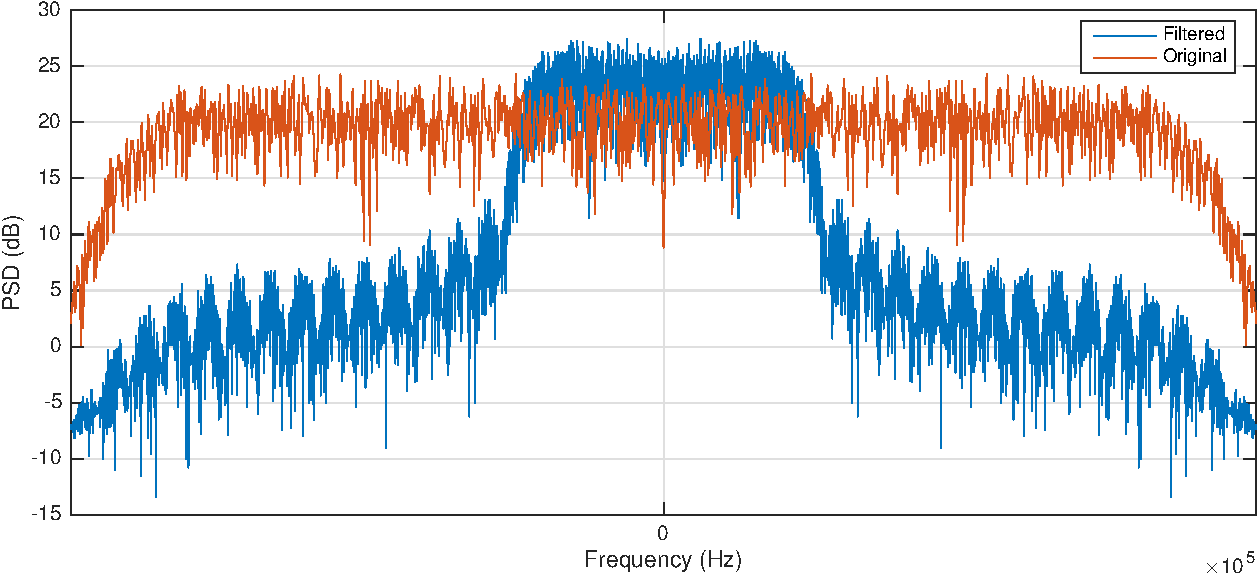
\includegraphics[width=0.5\textwidth]{bandlimiting-eps-converted-to-crop.pdf}
\caption{Frequency spectrum of PSK signal before and after pulse shaping.}
\label{fig:bandlimiting}
\end{figure} 
%
In previous labs and in previous chapters we have discussed matched filters and transmit filters.  We will 
revisit those topics again here to discuss how they are used in practices and demonstrate effects they help 
elevate.  In digital communications theory when matched filtering is discussed it is typically called pulse 
shaping at the transmitter and matched filtering at the receiver for reference.   The goal of these 
techniques is three fold: first to make the signal suitable to be transmitted through the communication channel mainly by limiting its effective bandwidth, increase the SNR of the received waveform, and to reduce intersymbol interference (ISI) from multi-path channels and nonlinearities.\par
%
By filtering a symbols sharp phase and frequency transitions are reduced, resulting in a more compact and 
spectrally efficient signal. Figure~\ref{fig:bandlimiting} provides a simple example of a DBPSK signal's frequency representation before and after filtering with a transmit filter.  The filter used to generate this figure was a square-root raised cosine (SRRC) filter, which is a common filtered use in communication system. We provide the  raised cosine filter in Chapter 2, but the more common SRRC has the impulse response:
%
\begin{equation}
	h(t) = \begin{cases}
 \dfrac{1}{\sqrt{T_s}} \left( 1-\beta+4\dfrac{\beta}{\pi} \right),
       & t = 0 \\

\dfrac{\beta}{\sqrt{2T_s}}
\left[
\left(1+\dfrac{2}{\pi}\right)\sin\left(\dfrac{\pi}{4\beta}\right) +
\left(1-\dfrac{2}{\pi}\right)\cos\left(\dfrac{\pi}{4\beta}\right)
\right],
       & t = \pm \dfrac{T_s}{4\beta} \\

\dfrac{1}{\sqrt{T_s}} \dfrac{\sin\left[\pi \dfrac{t}{T_s}\left(1-\beta\right)\right] + 4\beta\dfrac{t}{T_s}\cos\left[\pi\dfrac{t}{T_s}\left(1+\beta\right)\right]}{\pi \dfrac{t}{T_s}\left[1-\left(4\beta\dfrac{t}{T_s} \right)^2 \right]},
       & \mbox{otherwise}
\end{cases}
\end{equation}
%
where $T_s$ is the symbol period and $\beta \in \big[0,1\big]$ is the roll-off factor.\par
%
The SRRC is used since it is a Nyquist type filter, which produces zero ISI when sampled correctly~\cite{proakis2008}. We can demonstrate the effect of ISI by introducing a simple nonlinearity into the channel and consult the resulting eye diagrams which were introduced in Section 2.4.1.  Nonlinearities cause amplitude and phase distortions, which can happen when we clip or operate at the limits of our transmit amplifiers.  For more details on the used model consult~\cite{saleh1981}, but other models exists such as~\cite{boum2006}.  In Figure~\ref{fig:isi} of observe the effects of ISI as the eye becomes compressed and correct sampling becomes difficult to determine.  We will revisit ISI effects again when equalization is discussed in Chapter 8.\par
%
\begin{figure}[!ht]
 \centering
 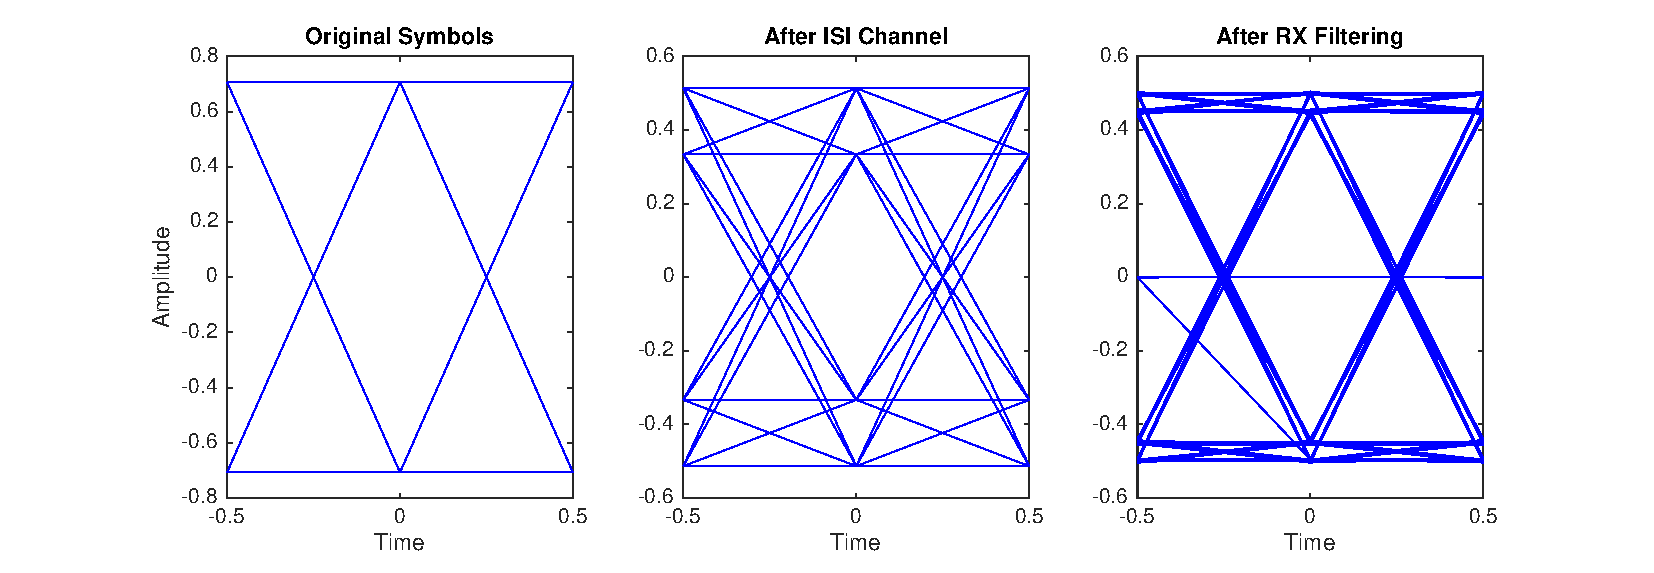
\includegraphics[width=0.9\textwidth]{isiExample.eps}
\caption{Eye diagrams of QPSK signal effected by nonlinearity causing ISI, which is reduced by SRRC matched filtering.}
\label{fig:isi}
\end{figure} 
%
The final aspect of the matched filters we want to discusses or provide insight into is SNR maximization.  This argument logically comes out of the concept of correlation.  Since the pulsed-shaped/filtered signal is correlated with the pulse shaped filter and not the noise, matched filtering will have the effect of SNR maximizing the signal.  Creating peaks at central positions of receive pulses.  We demonstrate this effect in Figure~\ref{fig:srrc}, where we present data transmitted with and without pulse shaping under AWGN.  In the middle plot we observe a signal closely related to the originally transmitted sequence, even under high noise.  However, without pulse shaping even visually the evaluation of the transmitted pulse becomes difficult.  We even observe demodulation errors in this third plot without anytime timing offset introduced.\par
%
\begin{figure}[!ht]
 \centering
 \includegraphics[width=0.9\textwidth]{filteredEffectsBest.eps}%{filteredEffectsSRRC-eps-converted-to-crop.pdf}
\caption{Comparison of pulse shaping and non-pulse shaping received signals under AWGN.}
\label{fig:srrc}
\end{figure} 
%

\subsection{Timing Error}
%
In the most basic sense the purpose of symbol timing synchronization is the align the clocking signals or 
sampling instances of two disjoint communicating devices.  In Figure~\ref{fig:clocking} we consider a simple example where we overlap the clocking signal and input signal to be sampled.  The sampling occurs at the rising clock edges, and the optimal timing is provided.  However, in a real-world environment there will some unknown non-zero delay or shift of the clocking signal which can result non-optimal sampling or even wrong decisions.\par
%
\begin{figure}[!ht]
 \centering
 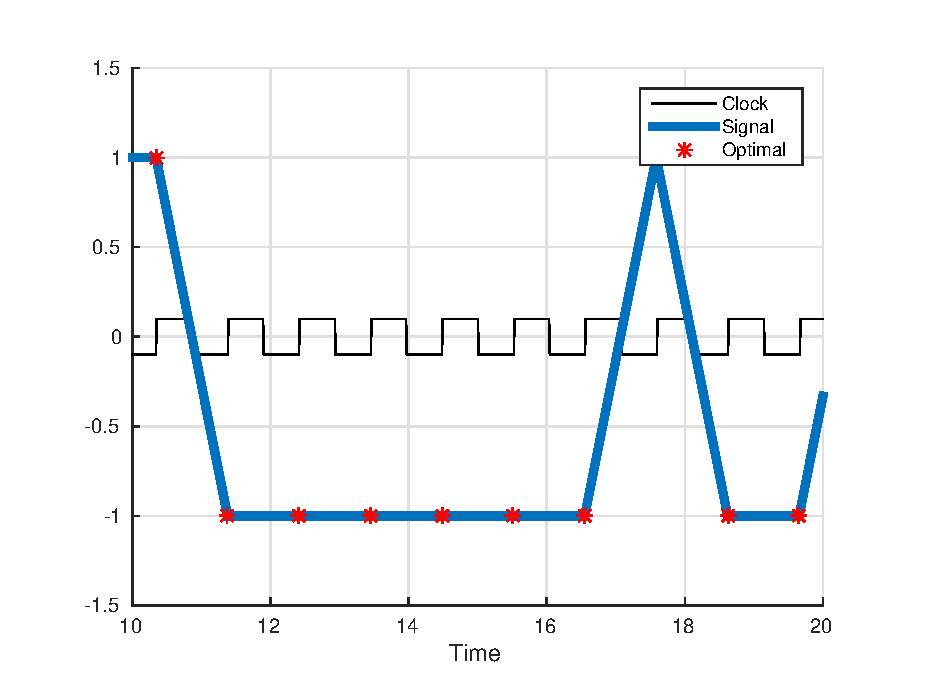
\includegraphics[width=0.5\textwidth]{clocking.eps}
\caption{Example received symbols and associated optimal clocking.}
\label{fig:clocking}
\end{figure} 
%
In the case of our wireless transmissions, if we consider this error from the perspective of the constellation diagram we will observe clustering or scattering of the symbols.  In Figure~\ref{fig:1}, we provide a simulated timing offsets of $0.2N$ and $0.5N$, where $N$ is the samples per symbol.  An offset of $0.5N$ is the worse case because we are exactly between two symbols.  In Figure~\ref{fig:2} we provide a QPSK transmitted through loopback of a single Pluto SDR.  We can clearly observe a similar clustering.\par  %The constellation appears rotated because the transmit and receive chain are out of phase with one-another.\par

\begin{figure}
\centering
  \begin{minipage}[b]{0.4\textwidth}
 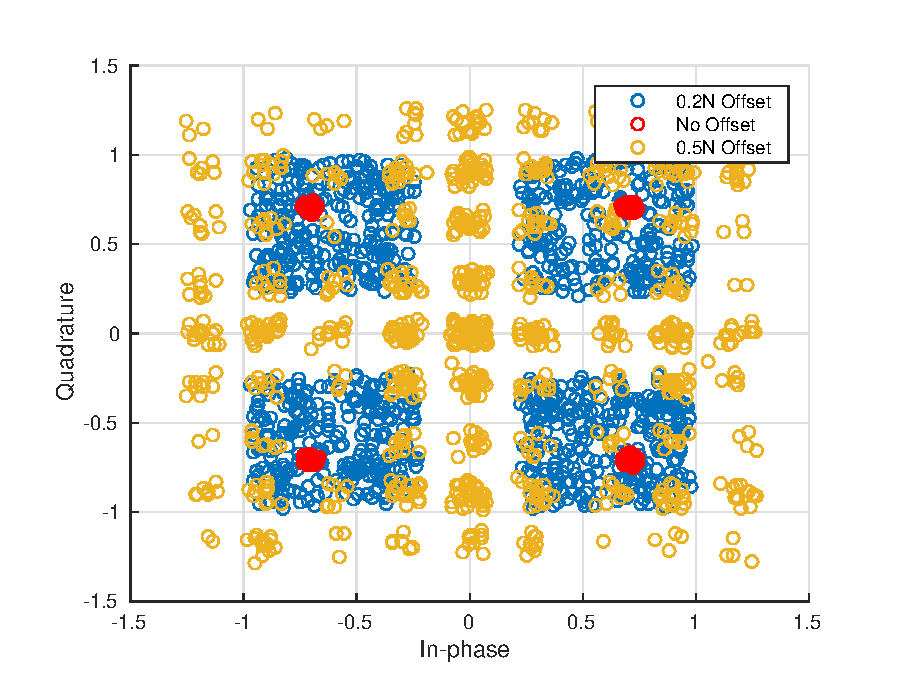
\includegraphics[width=\textwidth]{refConstellation.eps}
    \caption{Simulation example of timing offset effects on QPSK constellation.}
    \label{fig:1}
  \end{minipage}
  \begin{minipage}[b]{0.4\textwidth}
 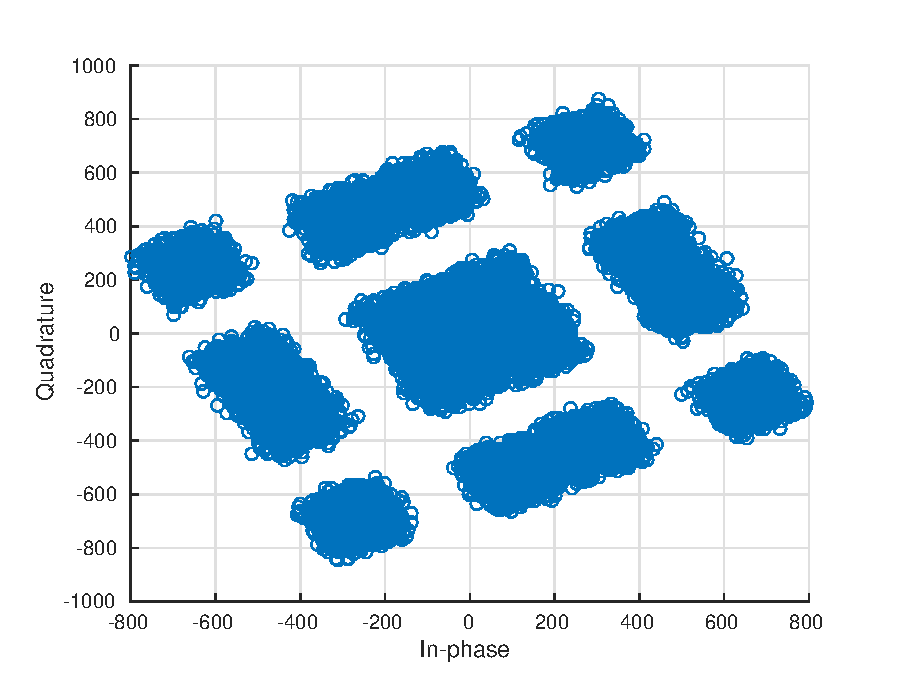
\includegraphics[width=\textwidth]{plutoConstellation.eps}
    \caption{Example with data sent through Pluto using a loopback cable.}
    \label{fig:2}
  \end{minipage}
\end{figure}

Mathematically we can model this offset input signal which has passed through the receive matched filter as:
%
\begin{equation}
	x(kT_s) = \sum_{n} x(n) p((k-n)T_s - \tau) + v(kT_s),
\end{equation}
%
where $p$ is the autocorrelation of the pulse shape use on the source data $x$, and $v$ is the shaped noise.  The unknown delay $\tau$ must 
be estimated to provide correct demodulation downstream.\\

\vbox{
\questionbox{
\begin{itemize}
  \item Question 0: Explain the difference between type I and type II Nyquist filters. 
  \item Question 1: Generate frequency response plots for SRRC filter realizations with $\beta \in\big[0, 0.1, 0.25, 0.5, 1\big]$.
  \item Question 2: Generate transmit and receive plots similar to Figure~\ref{fig:srrc} with $\beta \in\big[0.1, 0.5, 0.9\big]$ and discuss the time domain effects.
  \item Question 3: Compare and contrast the effects up-sample factor (samples per symbol) on the design of a communication system.
  \item Question 4: Regenerate Figure~\ref{fig:2} with data from your Pluto SDR and explain why the constellation appears rotated.  It may be helpful to start with \texttt{loopback.m} from Lab0.
\end{itemize}
}
}

\newpage
\section{Symbol Timing Compensation}\label{sec:timing}
%
There are many ways to perform correction for symbol timing mismatches between transmitters and
receivers. However, in this Chapter we will examine three digital phase lock loop (PLL) strategies which
will also share the same methodology as in Laboratory 2 for our carrier recovery implementations. This type of timing recovery was chosen because it can be integrated with our existing recovery solutions.  For the PLL outlined in Figure~\ref{fig:ts_pll}, we will first provide an overview conceptually how timing is synchronized, and then move into each individual block, explaining their design. The detectors discussed will be: zero-crossing, M\"{u}ller and Mueller, and Gardner.\par

\begin{figure}[!ht]
\centering
\begin{tikzpicture}[auto, node distance=2cm,>=latex']
    % Blocks and positions
    \node [input, name=input] {};
    \node [block, right of=input] (mf) {\begin{tabular}{c} Matched \\ Filter \end{tabular}};
    \node [block, right of=mf, node distance=3.5cm] (interpolator) {Interpolator};
    \node [block, below of=interpolator, node distance=3cm] (ic) {Controller};
    \node [block, right of=ic, node distance=3.5cm] (lf) {Loop Filter};
    \node [block, right of=lf, node distance=3.5cm] (ted) {TED};
    \node [outputMiddle, above of=ted, node distance=3cm] (outputMiddle) {};
    \node [output, right of=outputMiddle, node distance=1cm] (output) {};
    % Lines
    \draw [draw,->] (input) -- node {$r(t)$} (mf);
    \draw [draw,->] (mf) -- node {$y(t)$} (interpolator);
    \draw [-] (interpolator) -- node {$y(nT+\hat{\tau})$} (outputMiddle);
    \draw [->] (outputMiddle) -- node {} (output);
    \draw [->] (outputMiddle) -- node {} (ted);
    \draw [->] (ted) -- node {$e(n)$} (lf);
    \draw [->] (lf) -- node {$g(n)$} (ic);
    \draw [->] (ic) -- node {} (interpolator);
\end{tikzpicture}
\caption{Basic structure of PLL for timing recovery.}
\label{fig:ts_pll}
\end{figure}

The timing synchronization PLL used in all three algorithms consists are four main blocks: interpolator, 
timing error detector (TED), loop filter, and an interpolator controller.  This all-digital PLL-based algorithm shown here works by first measuring an unknown offset error, scale the error proportionally, and apply an update 
for future symbols to be corrected. To provide necessary perspective on the timing error, let us considered 
the eye diagram presented in Figure~\ref{fig:eye_tm}.  This eye diagram has been up-sampled by twenty times so 
we can examine the transitions more closely, which we notice are smooth unlike Figure~\ref{fig:isi}.  In the optimal case, we chose to ``sample'' our input signal at the red instances at the widest openings of the eye.  However, there will be an unknown fractional delay $\tau$ which shifts this sampling period.  This shifted sampling position is 
presented by the green selections. To help work around this issue, our receive signal is typically not 
decimated fully, providing the receiver with multiple samples per symbol (This is not always the case). 
Therefore, if we are straddling the optimal sampling position instead as in the black markers.  We can simply 
interpolate across these points to get our desired period.  This interpolation has the effect of causing a 
fractional delay to our sampling, essentially shifting to a new position in our eye diagram. Since $\tau$ is 
unknown we must weight this interpolation correctly so we do not overshoot or undershoot the desired 
correction.\par
%
\begin{figure}
 \centering
 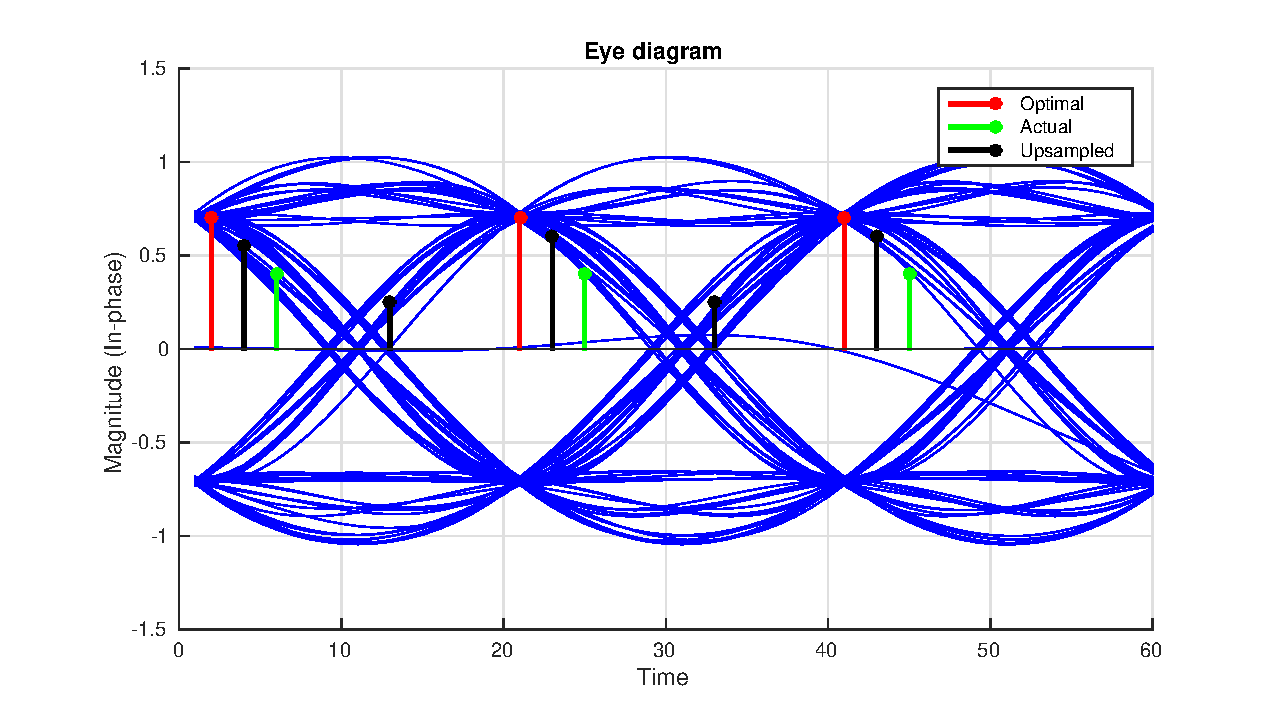
\includegraphics[width=0.8\textwidth]{eyeDiagram.eps}
\caption{}
\label{fig:eye_tm}
\end{figure} 
%
We will initially discuss the specifics of the blocks in Figure~\ref{fig:ts_pll} through the perspective of 
the zero-crossing (ZC) method, since it is the most straight forward to understand.  Then we will provide 
extensions to the alternative methods. In ZC as the name suggests, will produce an error signal of zero when 
one of the sampling positions is at the zero intersection.  ZC requires two samples per symbol, resulting in 
the other sampling position occurring at or near the optimal position.  The TED for ZC~\cite{mengali1997synchronization} is 
evaluated as:
%
\begin{equation}\label{eq:zc_ped}
\begin{split}
  e(k) =\, & Re( x((k-1/2)T_s + \tau ) )\big[sgn\{Re(x((k-1)T_s + \tau ))\} - sgn\{Re(x(kT_s + \tau 
))\}\big] + \\
  &Im( x((k-1/2)T_s + \tau ) )\big[sgn\{Im(x((k-1)T_s + \tau ))\} - sgn\{Im(x(kT_s + \tau ))\}\big].
\end{split}
\end{equation}
%
Note that these indexes are with respect to symbols, not samples.  Equation~\eqref{eq:zc_ped} first provides 
a direction for the error with respect to the $sgn$ operation, and the shift required to compensate is 
determined by the midpoints.  The in-phase and quadrature portions operate independently, which is 
desirable. Once the error is calculated it is passed to the loop filter:%, which we can entirely borrow from our 
%discussion on carrier recovery.  The same principles apply here, with a near identical formulation for our 
%equations we have provided in a slightly more compact form.
\begin{equation}
  \theta = \frac{B_{Loop}}{M(\zeta + 0.25/\zeta)} \quad \quad \Delta = 1 + 2\zeta\theta + \theta^2
\end{equation}
\begin{equation}
  G_1 = \frac{-4\zeta\theta}{G_D N\Delta} \quad \quad G_2 = \frac{-4\theta^2}{G_D N\Delta}
\end{equation}
%
Here $B_{Loop}$ is the normalized loop bandwidth, $\zeta$ is our damping factor, $N$ is our samples per symbol, and $G_D$ is our detector gain.  The new variable $G_D$ provide an additional step size scaling to our correction.  Again the loop filter's purpose is maintain stability of the correction rate.  This filter can be implemented with a simple linear equation:
\begin{equation}
	y(n) = G_1x(n) + G_2 \sum_{k=0}^{n}x(k),
\end{equation}
or with a Biquad filter.
\par
%
The next block to consider is the interpolation controller, which is responsible to providing the necessary 
signaling to the interpolator.  Since the interpolator is responsible for fractionally delaying the signal, 
this controller must provide this information and generally the starting interpolant sample.  By starting 
interpolant sample we are referring to the sample on the left side of the straddle, as shown by the second 
black sampling position from the left in Figure~\ref{fig:eye_tm}.  The interpolation controller implemented here 
will utilize a counter-based mechanism to effectively trigger or \textit{strobe} at the appropriate symbol 
positions. At these strobe positions is when the interpolator is signaled and updated.\par
%
The main idea behind a counter-based controller is to maintain a specific triggering gap between updates to the interpolator, with an update period on average equal to symbol rate.  If we consider the case when the timing is optimal and the output of the loop filter $v(n)$ is zero, we would want to produce a trigger every $N$ samples.  Therefore, it is logical that the weighting or decrement for the counter would be:
%
\begin{equation}
 W(n) = v(n) + \frac{1}{N}.
\end{equation}
%
Resulting in a maximum value of $1$ under modulo-$1$ subtraction of the counter $c(n)$, where wraps of the modulus occur every $N$ subtractions.  This modulus counter update is defined as:
%
\begin{equation}
 c(n+1) = (c(n) -W(n))\mod{1}.
\end{equation}
%
We determine a strobe condition, which is checked before the counter is updated, based on when these modulus wraps occur.  We can easily check for this condition before the update such as:
%
\begin{equation}
 Strobe = \begin{cases}
 c(n) < W(n) & True \\ 
\mbox{Otherwise} & False \end{cases}.
\end{equation}
%
This strobing signal is the method used to define the start of a new symbol, therefore it can also be used to make sure we are estimating error over the correct samples.  When the strobe occurs we will updated $\mu(n)$ our estimated gap between the interpolant point and the optimal sampling position.  This update is a function of the new counter step $W(n)$ and our current count $c(n)$:
%
\begin{equation}
	\mu(k) = c(n)/W(n).
\end{equation}
%
This $\mu$ will be passed to our interpolator to update the delay it applies.\par
%
We want to avoid performing timing estimates that span over multiple symbols, which would provide incorrect error signals and incorrect updates for our system.  We can avoid this by adding conditions into the TED block.  We provide additional structure to the TED block in Figure~\ref{fig:ted}, along with additional logic to help identify how we can effectively utilize our strobe signals.  Based on this TED structure, only when a strobe occurs the output error $e$ can be non-zero.  Looking downstream, since we are using a PI loop filter only non-zero inputs can update the output, and as a result modify the period of the strobe $W$.  When the system enters steady state, where the PLL has locked, the TED output can be non-zero every $N$ samples.\par
%

\begin{figure}[!ht]
\centering
\begin{tikzpicture}[auto, node distance=1.5cm,>=latex']
     % Blocks and positions
     \node [input, name=input] {};
     \node [block, right of=input, node distance=3cm] (interpolator) {Interpolator};
     \node [outputMiddle, right of=interpolator, node distance=9cm] (outputMiddle) {};
     \node [output, right of=outputMiddle, node distance=1cm] (output) {};
     \node [block, below of=outputMiddle, node distance=3cm] (ted) {TED};
     \node [block, below of=ted, node distance=3cm] (lf) {Loop Filter};
     \node [circle, draw, left of=lf, node distance = 3cm] (sum) {+};
     \node [block,minimum width=1cm, above of=sum, node distance = 1.5cm] (const) {$\frac{1}{N}$};
     \node [diamond, draw, fill=blockcolor, left of=sum, node distance=3cm] (counter) {$d(n) > c(n)$};
     \node [block, above of=counter, node distance=3cm] (updater) {\begin{tabular}{c} Update\\Taps ($\mu$)\end{tabular}};
     \node [block, below of=interpolator, node distance=1.5cm] (updatecount) {\begin{tabular}{c} Update\\$c$ \end{tabular}};
     \node [block, right of=updatecount, node distance=3cm] (trigger) {\begin{tabular}{c} Enable\\Trigger \end{tabular}};
     % Lines
     \draw [draw,->] (input) -- node {$y(nT)$} (interpolator);
     \draw [-] (interpolator) -- node {$y(nT+\hat{\tau})$} (outputMiddle);
     \draw [->] (outputMiddle) -- node {} (output);
     \draw [->] (outputMiddle) -- node {} (ted);
     \draw [->] (ted) -- node {$e(n)$} (lf);
     \draw [->] (lf) -- node {$\quad p(n)$} (sum);
     \draw [->] (sum) -- node {$d(n)$} (counter);
     \draw [->] (counter) -- node {Yes} (updater);
     \draw [->] (updatecount) -- node {} (interpolator);
     \draw [->] (trigger) -- node {} (updatecount);
     \draw [->] (counter) -| node {No} (updatecount);
     \draw [->] (const) -- node {} (sum);
     \draw [->] (updater) -- node {} (trigger);
     % Draw box
     \node[dashed,draw,inner sep=2mm,label=below:Interpolation Controller,fit=(updatecount) (counter) (const) (updatecount)] {};
 \end{tikzpicture} 
 \caption{Timing recovery triggering logic used to maintain accurate interpolation of input signal.}
 \label{fig:ted}
 \end{figure}
  \begin{figure}[!ht]
  \centering
   \begin{tikzpicture}[auto, node distance=1.5cm,>=latex']
      % Blocks and positions
      \node [input, name=input] {};
      \node [diamond, fill=blockcolor, draw, right of=input, node distance=4cm] (tedcheck) {Trigger?};
      \node [block, below of=tedcheck, node distance=3cm] (calculate_e) {Calculate $e(n)$\\From $y(nT)$};
      \node [block, right of=tedcheck, node distance=3cm] (e_zero) {$e(n)=0$};
      \node [output, right of=e_zero, node distance=2cm] (output) {};
      \node [output, right of=output, node distance=2cm] (outputEnd) {};
      %\node [output, right of=e_zero, node distance=3cm] (output_zero) {};
      % Lines
      \draw [draw,->] (input) -- node {$y(nT+\hat{\tau})$} (tedcheck);
      \draw [->] (tedcheck) -- node {No} (e_zero);
      \draw [->] (tedcheck) -- node {Yes} (calculate_e);
      \draw [-] (e_zero) -- node {} (output);
      \draw [-] (calculate_e) -| node {} (output);
      \draw [->] (output) -- node {$e(n)$} (outputEnd);
      % Draw box
      \node[dashed,draw,inner sep=2mm,label=below:TED,fit=(tedcheck) (calculate_e) (output) (tedcheck)] {};
  \end{tikzpicture}
  \caption{ An internal view of the timing error detector to outline the error and triggering control
signals relation to operations of other blocks in Figure~\ref{fig:ted}}
 \end{figure}
%

The final piece of the timing recovery we have not yet discussed is the interpolator itself.  Interpolation is simply a linear combination of the current and past inputs $x$, which in essence can be though of as a filter.  However, to create a FIR filter with any arbitrary delay $\tau \in \big[0,...,T_s\big]$ cannot be realized~\cite{unitDelay}.  Realizations for ideal interpolation IIR filters do exist, but the computation of their taps are impractical in real systems~\cite{Thiran1971}.  Therefore, we will use an adaptive implementation of a FIR lowpass filter called a piecewise polynomial filter (PPF)~\cite{rice2009}.  The PPF can only provide estimations of offsets to a polynomial degree.  Alternative implementations exists such as polyphase-filterbank designs, but depending on the required resolution the necessary phases become large.\par
%
The PPF are useful since we can easily control the form of interpolations by determining the order of the filter, which at most is equivalent to the order of the polynomial used to estimate the underlying received signal.  Here we will use a second order, or quadratic, interpolation requiring a four tap filter.  The general form of the interpolator's output is given by:
%
\begin{equation}\label{eq:ppf_eq}
 x(kT_s + \mu(k)T_s) = \sum_{n=-2}^{1} h(n) x((k-n)T_s),
\end{equation}
%
where $h_k$ are the filter coefficients at time instance $k$ determined by~\cite{harris1993}:
%
\begin{equation}
\begin{split}
 h = &[\alpha\mu(k)(\mu(k)-1),\\
 &-\alpha\mu(k)^2-(1-\alpha)\mu(k) + 1,\\
 &-\alpha\mu(k)^2+(1+\alpha)\mu(k) ,\\
 &\alpha\mu(k)(\mu(k)-1)],\\
\end{split}
\end{equation}
%
where $\alpha=0.5$. $\mu(k)$ is the fractional delay which is provided by the interpolator control block, which relates the symbol period $T_s$ to the estimated offset.  Therefore, we can estimate the true delay $\tau$ as:
%
\begin{equation}
	\hat{\tau} = \mu(k)T_s.
\end{equation}
%
Without any offset ($\mu=0$), the interpolator acts as a two sample delay or single symbol delay for the ZC implementation.  We can extend the PPF to utilize more samples creating cubic and greater interpolations, but there implementations by become more complex.  The underlying waveform should be considered when determining the implementation of the interpolator, and the required degrees of freedom to accurately capture the required shape.\par
This design using four samples in a quadratic form can be considered irregular, since the degree of taps does not reach $3$.  However, odd length realizations (using an odd number of samples) are not desirable since we are trying to find values in-between the provided samples.  We also do not want a $2$ sample implementation due to the curvature of the eye in Figure~\ref{fig:eye_tm}.\par 
%
The overall design of the synchronizer can be complex and implementations do operate at different relative rated.  Therefore, we have provided Table~\ref{my-label} on guide of a recommended implementation.  These rates align with the strobe implementation outlined in Figure~\ref{fig:ted}. This system will result in one sample per symbol when output samples of the interpolator are aligned with the strobes.

%
%\begin{figure}
\begin{table}[!ht]
\centering
\caption{Operational Rates of Timing Recovery Blocks}
\label{my-label}
\begin{tabular}{l|l}\hline
 Block & Operational Rate \\ \hline
 Interpolator & Sample Rate \\
 TED & Symbol Rate \\
 Loop Filter & Symbol Rate \\
 Interpolator Controller & Sample Rate 
\end{tabular}
\end{table}
%\end{figure}
%


\subsection{Gardner}\label{sec:gard}
%
The second TED we will considered is called Gardner~\cite{gardner1986}, which is very similar to ZC.  The error signal is determined by:
%
\begin{equation}\label{eq:ga_ted}
\begin{split}
  e(k) =\, & Re( x((k-1/2)T_s + \tau ) )\big[Re(x((k-1)T_s + \tau )) - Re(x(kT_s + \tau 
))\big] + \\
  &Im( x((k-1/2)T_s + \tau ) )\big[Im(x((k-1)T_s + \tau )) - Im(x(kT_s + \tau ))\big].
\end{split}
\end{equation}
%
This method also requires two samples per symbol and differs only in the quantization of the error direction from ZC.  One useful aspect of Gardner is that it does not require carrier phase correction and works specifically well with BPSK and QPSK signals.  However, since Gardner is not a decision directed method for best performance the excess bandwidth of the transmit filters should be $\beta \in \big(0.4,1\big)$.

\subsection{M\"{u}ller Mueller}\label{sec:mm}
%
Next is the M\"{u}ller and Mueller (MM) method named after Kurt Mueller and Markus M\"{u}ller~\cite{mm1976}.  This can be considered the most efficient method since it does not require upsampling of the source data, operating at one sample per symbol. The error signal is determined by~\cite{rice2009}:
%
\begin{equation}\label{eq:ga_ted}
\begin{split}
  e(k) &= Re( x((k)T_s + \tau ) )sgn\{Re(x((k-1)T_s + \tau ))\} \\
  & - Re( x((k-1)T_s + \tau ) )sgn\{Re(x((k)T_s + \tau ))\} \\
  & + Im( x((k)T_s + \tau ) )sgn\{Im(x((k-1)T_s + \tau ))\} \\
  & - Im( x((k-1)T_s + \tau ) )sgn\{Im(x((k)T_s + \tau ))\} \\
\end{split}
\end{equation}
%
MM also operates best when the matched filtering used minimizes the excess bandwidth.  When the excess bandwidth is high the decisions produce by the $sgn$ operation can be invalid.\par


\vbox{
\questionbox{
\begin{itemize}
  \item Question 0: Starting with \texttt{lab1.m}, which demonstrates a slowly changing timing offset, implement in MATLAB either the ZC, MM, or Gardner timing correction algorithm.
  \item Question 1: Provide EVM measurements of the signal before an after your timing correction at different noise levels.
  \item Question 2: Introduce a fixed phase offset and repeat your EVM measurements from Question 1.
\end{itemize}
}
}

\section*{Implementation Guidance}
\begin{itemize}
	\item A recommended starting configuration for your loop filter should be $\big[N, \zeta, B_{Loop}, G_D \big] = \big[2, 1, 0.1, 2.7 \big]$.
	\item Remove noise sources and then reintroduce them once your implementation becomes functional.
	\item Bit stuffing/removal is not discussed, but is simple to add.  These are required when you receive two strobes one after the other at the sample rate, which should not occur.  In this case introduce an extra zero into your TED input buffer, forcing an error calculation across at least one zero. This should not really happen in simulation since there is no jitter, but for more information consult~\cite[pg. 491]{rice2009}.
\end{itemize}


\section{Adding Pieces Together}\label{sec:combined}
%
Throughout this laboratory we have outlined the structure and logic behind a PLL based timing recovery algorithm and the associated MATLAB code. In the remaining laboratories we will discuss putting the algorithmic components together and provide some intuition on what happens during evaluation. Here we will also address parameterization and the relation to system dynamics. The system level scripts have shown a constant theme throughout where data is modulated, transmit filtered, passed through a channel with timing offset, filtered again, then is timing recovered. Many rate changes can happen in this series of steps. To help understand these relations better we can map things out as in Figure~\ref{timecorr}, which takes into account these stages. Here the modulator produces symbols equal to the sample rate. Once passing through the transmit filter we acquire our upsampling factor $N$ , which increases our samples per symbol to $N$ . At the receiver we can perform decimation in the receive filter, by a factor $N_F$ where $N_F \leq N$ . Finally, we will perform timing recovery across the remaining samples and
remove the fractional offset $\tau$ , returning to the original rate of one sample per symbol.
%
\begin{figure}[!ht]
\centering
  \begin{tikzpicture}[auto, node distance=2cm,>=latex']
      % Blocks and positions
      \node [input, name=input] {};
      \node [block, right of=input, node distance=4cm] (mod) {Modulator};
      \node [block, right of=mod, node distance=4cm] (txfilt) {Transmit Filter};
      \node [block, right of=txfilt, node distance=4.5cm] (chan) {Channel w/ Offset};
      \node [block, below of=txfilt, node distance=2cm] (rxfilt) {Receive Filter};
      \node [block, left of=rxfilt, node distance=5cm] (timerec) {Timing Recovery};
      \node [output, left of=timerec, node distance=4cm] (output) {};
      % Lines
      \draw [draw,->] (input) -- node {data} (mod);
      \draw [->] (mod) -- node {$T_s$} (txfilt);
      \draw [->] (txfilt) -- node {$NT_s$} (chan);
      \draw [->] (chan) |- node {$NT_s+\tau^{*}$} (rxfilt);
      \draw [->] (rxfilt) -- node {$\frac{N}{N_F}T_s+\tau^*$} (timerec);
      \draw [->] (timerec) -- node {$T_s$} (output);
  \end{tikzpicture} 
  \caption{Relative rates of transmit and receive chains with respect to the sample rate at different
stages. Here $\tau^*$ represents a timing shift not an increase in the data rate. This is a slight abuse of notation.}
\label{timecorr}
\end{figure}
%
\vbox{
\questionbox{
\begin{itemize}
  \item Question 0: Provide your chosen arrangement of recovery blocks and reasoning behind their selected placement.
  \item Question 1: With your new receive chain, generate a received signal (before the receive filter in Figure~\ref{fig:srrc}) under the following conditions and provide EVM measurements after timing recovery:
  \begin{enumerate}
    \item No offsets
  	\item A fixed timing offset
  	\item A fixed phase offset
  \end{enumerate}
  Provide results over a small range of SNRs.
\end{itemize}
}
}


\newpage
\section{Open-ended Design Problem: Automatic Timing Compensation With Pluto}

%NEW SYSTEM DIAGRAM WITH SYNCHRONIZERS
%
%COMBINE COARSE AND FINE FREQUENCY CORRECTION IS APPROPRIATE FASHION AND DESCRIBE REASONING


\subsection{Objective}
The objective of this problem is to design and implement a
software-defined radio (SDR) communication system capable of
automatically calculating and correcting the timing offsets between two Pluto
SDRs.

In Sections~\ref{sec:timing} you have implemented and simulated timing correction.  
Now we will introduce the Pluto to deal with realistic timing behavior.  To simplify this process a set of required tasks are staged to gradually increase the difficulty of the overall implementation.  We have presented threee methods for timing correction, but you are free to use these in any arrangement you want, or use your own algorithms.  However, you must 
provide an evaluation of the overall system performance.  Your final implementation should be tuned to handle 
any set of Pluto radios, not just the ones used by your team.\par
%
With your built frequency correction code perform the following tasks:
%
\begin{enumerate}
 \item First, using a single Pluto transmit your DBPSK or QPSK reference signal across to the same radio.  It may be useful to start with the \texttt{loopback.m} example provided in Lab 0.  This will provide you will minimal to zero frequency offset.  Therefore, you will only have to compensate for phase and timing.  Graph the resulting baseline EVM.
\item Repeat this experiment by increasing the center frequency of the transmit or receive chain.  Graph the resulting EVM.
  \item Third, using a pair of Plutos repeat this estimation again as previously performed with a single 
Pluto.  Provide EVM measurements at different distances and/or different gain setting for the radio.
  \item Compare your results here from what you have obtained in Sections~\ref{sec:combined} in a way you determine as appropriate.
\end{enumerate}
%

% \subsection{Theoretical Background}
% \begin{enumerate}
% \item Before you apply your method to USRP2 boards, it is highly recommended that you test your method with Simulink-only model without USRP and see whether it works.
% \item In the Simulink-only model, you can introduce the frequency offset by \texttt{Phase/Frequency Offset} block. Specify a frequency offset in this block, and see whether
% your Simulink model can give you the number you have specified.
% \item An important hint: If you take the square of a signal, the FFT of the received signal will be shifted double of the frequency offset.
% \item In your model, you might need the following blocks:
% \begin{enumerate}
% \item \texttt{Random Integer Generator}
% \item \texttt{Baseband Modulator}
% \item \texttt{Raised Cosine Transmit Filter}
% \item \texttt{Magnitude FFT}
% \item \texttt{Probe}
% \item \texttt{Maximum}
% \end{enumerate}
% The first three blocks are used on the transmitter side, and the
% last three blocks are used on the receiver side. Using
% \texttt{Probe} and \texttt{Maximum}, you will be able to find the
% location of the peak of the FFT. But of course, you are not
% constrained to these blocks. You can use all the blocks available in
% Simulink. If you want, you can even use MATLAB to implement your
% method.
% \item Although you are required to find the frequency offset of two USRP2 boards, you are actually trying to find the frequency offset of the received signal.
% \item Compare your result here from what you have obtained in Section~\ref{sec:offset}.
% \end{enumerate}
%
% \newpage

\section{Lab Report Preparation \& Submission Instructions}
Include all your answers, results, and source code in a laboratory
report formatted as follows:
\begin{itemize}
 \item Cover page: includes course number, laboratory title, names and student numbers of team, submission
 date.
 \item Table of contents, list of tables, list of figures.
 \item Commentary on designed implementations, responses to laboratory questions, and explanation of
 observations.
 \item Responses to open-ended design problem.
 \item Source code (as an appendix).
\end{itemize}

Remember to write your laboratory report in a narrative approach, explaining your experience and observations in such a way that it provides the reader with some insight as to what you have accomplished.  Furthermore, please include images and outputs wherever possible in your laboratory report document.\\

\noindent Each group is required to submit a single report
electronically (in PDF format) to \texttt{alexw@wpi.edu} by the scheduled due date and time.
Reports that do not meet these specifications will be returned
without evaluation and will receive a grade of ``0'' for the report
segment of the laboratory experiment.


\newpage
\bibliographystyle{plain}
\bibliography{lab1bib}


\end{document}
